\documentclass[12pt]{article}
\usepackage[utf8]{inputenc}
\usepackage{geometry}
\usepackage{graphicx}
\usepackage{hyperref}
\usepackage{amsmath}
\usepackage{amsfonts}
\usepackage{listings}
\usepackage{xcolor}
\usepackage{float}
\usepackage{longtable}
\usepackage{array}
\usepackage{tabularx}
\usepackage{booktabs}
\usepackage{caption}
\usepackage{url}
\usepackage{tikz}
\usetikzlibrary{matrix, shapes, arrows.meta, positioning, decorations.pathreplacing}
\usepackage[document]{ragged2e}
\usepackage{chronology}

% Document geometry
\geometry{a4paper, margin=1in}

\title{
    {\Huge Module Guide for Angry Birds Alike} \\
    {\Large Author: Al Jubair Hossain} \\
    {\large Date: March 31, 2024}
}
\date{}

\begin{document}

\maketitle

\newpage

\section*{Revision History}
\begin{longtable}{|p{2cm}|p{2cm}|p{10cm}|}
    \hline
    \textbf{Date} & \textbf{Version} & \textbf{Notes} \\
    \hline
    March 4, 2023 & 1.0 & Fixed hyperlink. \\\hline
    March 12, 2023 & 1.0 & Changed section 7. \\\hline
    March 31, 2023 & 1.5 & Updates to the Module Guide sections of 3, 4, 5, 6, 7 added hierarchy betweem modules, hierarchy diagrams and relation of TC between SRS, VnV Plan, added a UI section with diagrams based on initial implementation feedback. \\
    \hline
\end{longtable}

\newpage

\tableofcontents

\newpage

\section{Reference Material}
This section records information for easy reference.

\subsection{Table of Abbreviations and Acronyms}
\begin{longtable}{|l|l|}
    \hline
    \textbf{Abbreviation/Acronym} & \textbf{Description} \\
    \hline
    AC & Anticipated Change \\
    DAG & Directed Acyclic Graph \\
    M & Module \\
    MG & Module Guide \\
    OS & Operating System \\
    R & Requirement \\
    SC & Scientific Computing \\
    SRS & Software Requirements Specification \\
    ProgName & Angry Birds Alike, the name of the game developed \\
    UC & Unlikely Change \\
    \hline
\end{longtable}


\section{Introduction}

Decomposing a system into modules is a widely accepted approach to developing software. A module can be thought of as a work assignment for a programmer or programming team. We adopt a decomposition strategy based on the principle of information hiding, as suggested by Parnas (1972). This principle supports the design for change, as the "secrets" each module conceals are those aspects of the system most likely to change. This approach is particularly valuable in software development environments where modifications are frequent.

For "Angry Birds Alike", the module design has been constructed to adapt to changes with minimal impact on the overall system. Our design adheres to the rules set out by Parnas and colleagues (1984):

\begin{itemize}
    \item System details that are likely to change independently are the "secrets" of separate modules.
    \item Each data structure is encapsulated within a single module.
    \item Access to a module's data structure is only possible through its defined interface.
\end{itemize}

Following the completion of the Software Requirements Specification (SRS) and Verification and Validation Plan, we developed this Module Guide (MG). The MG delineates the system's modular structure, allowing designers and maintainers to identify software components efficiently.

Intended readers of this document include:

\begin{itemize}
    \item \textbf{New project members:} To provide a comprehensive overview of the system architecture, facilitating a quicker onboarding process.
    \item \textbf{Maintainers:} To improve understanding of the system's modular structure for efficient maintenance and enhancement activities.
    \item \textbf{Designers:} To use the MG as a tool for verifying the system's consistency, feasibility, and adaptability to changes.
\end{itemize}

The design for "Angry Birds Alike" emphasizes modularity, anticipating the potential evolution of both software and hardware environments. The subsequent sections will detail the anticipated and unlikely changes, module hierarchy, and the connections between the system's requirements and its design.

\section{Anticipated and Unlikely Changes}

\subsection{Anticipated Changes}
The following anticipated changes are based on expected software evolution and feedback cycles during development:

\begin{itemize}
    \item AC1: The operating systems on which the software will run, potentially including Windows, macOS, iOS, and Android.
    \item AC2: Changes in the graphics engine to support enhanced visual effects or to improve performance on varying hardware specifications.
    \item AC3: Adjustments to the physics engine calculations to increase accuracy or efficiency as new computational methods are developed.
    \item AC4: Modifications to the user interface to improve user experience or to add new features.
    \item AC5: Updates to the network communication protocols to maintain security standards and improve multiplayer features.
    \item AC6: The introduction of new game levels, characters, or objects that require additional modules or changes to existing ones.
\end{itemize}

\subsection{Unlikely Changes}
The following aspects of the software are considered stable and unlikely to change:

\begin{itemize}
    \item UC1: The fundamental game mechanics of launching projectiles at targets, as this is central to the game's identity.
    \item UC2: The basic concept of using a slingshot as the primary interaction method for the user to control projectiles.
    \item UC3: The core concept of the game, which involves physics-based puzzles to be solved by the user, will remain unchanged.
    \item UC4: The software's reliance on the SFML library for rendering graphics and handling user input.
    \item UC5: The use of the C++ programming language and Boost libraries for the development of the game's core functionalities.
\end{itemize}

The identification of these anticipated and unlikely changes ensures that the modular design can accommodate future evolution while maintaining the core gameplay that defines "Angry Birds Alike."

\section{Module Hierarchy}

This section provides an overview of the modular design of "Angry Birds Alike." The hierarchy is decomposed by "secrets," as per Parnas's principle of information hiding. The design emphasizes modularity, facilitating easy updates and maintenance.

\subsection{Top-level Module Breakdown}
The following is a simplified view of the module hierarchy, focusing on the primary components of the game:

\begin{enumerate}
    \item M1: Hardware-Hiding Module
    \item M2: Behavior-Hiding Modules
        \begin{enumerate}
            \item M2.1: Game Logic Module
            \item M2.2: User Interface Module
        \end{enumerate}
    \item M3: Software Decision Module
        \begin{enumerate}
            \item M3.1: Physics Engine Module
            \item M3.2: Graphics Rendering Module
            \item M3.3: Input Handling Module
        \end{enumerate}
\end{enumerate}

\subsection{Detailed Module Descriptions}

\textbf{M1: Hardware-Hiding Module}
\textit{Secrets:} The details of hardware interaction.
\textit{Services:} Abstracts the hardware specifics from the rest of the software, allowing the game to run on various platforms without modification.
\textit{Implemented By:} Operating System and SFML library.

\textbf{M2: Behavior-Hiding Modules}
\textit{Secrets:} The specifics of the user interactions and game rules.
\textit{Services:} Provides the game's external behaviors as per the requirements, including game mechanics and user interactions.
\textit{Implemented By:} "Angry Birds Alike" software.

\textbf{M2.1: Game Logic Module}
\textit{Secrets:} The rules and mechanics of the game.
\textit{Services:} Manages the game state, including level progression, scoring, and gameplay mechanics.
\textit{Implemented By:} Game.cpp, Entity.cpp.

\textbf{M2.2: User Interface Module}
\textit{Secrets:} The structure and layout of the game's user interface.
\textit{Services:} Handles the rendering of the game's UI and captures user input.
\textit{Implemented By:} Game.cpp, utilizing SFML for rendering.

\textbf{M3: Software Decision Module}
\textit{Secrets:} The algorithms and data structures that do not directly interact with the game's behaviors.
\textit{Services:} Supports the behavior-hiding modules with necessary computational and storage mechanisms.
\textit{Implemented By:} "Angry Birds Alike" software.

\textbf{M3.1: Physics Engine Module}
\textit{Secrets:} The mathematical models and algorithms for simulating physics.
\textit{Services:} Simulates realistic physics for the game, including projectile motion and collisions.
\textit{Implemented By:} Physics.cpp, using Boost Odeint for numerical integration.

\textbf{M3.2: Graphics Rendering Module}
\textit{Secrets:} The methods for drawing graphics on the screen.
\textit{Services:} Renders the game's graphics, including entities and the UI.
\textit{Implemented By:} SFML library.

\textbf{M3.3: Input Handling Module}
\textit{Secrets:} The handling of user inputs.
\textit{Services:} Captures and processes user inputs to control the game.
\textit{Implemented By:} SFML library within Game.cpp.

This hierarchy facilitates a clear separation of concerns within the software, promoting maintainability and scalability. Each module's "secrets" denote areas of potential change, ensuring that modifications can be made with minimal impact on other parts of the system.

\section{Connection Between Requirements and Design}

This section outlines how the design of "Angry Birds Alike" satisfies the specific requirements identified in the Software Requirements Specification (SRS). The system's modular structure is directly influenced by these requirements, ensuring that each component of the game fulfills a distinct set of criteria.

\subsection{Requirements to Module Mapping}

The design decisions taken in the module structure are directly derived from the needs and functionalities described in the SRS. Below is a table mapping the main requirements of the system to the modules that implement them:

\begin{table}[H]
\centering
\begin{tabular}{|l|l|}
\hline
\textbf{Requirement} & \textbf{Responsible Module(s)} \\
\hline
Game Physics Simulation & M3.1: Physics Engine Module \\
User Interaction & M2.2: User Interface Module, M3.3: Input Handling Module \\
Graphics Rendering & M3.2: Graphics Rendering Module \\
Level Progression & M2.1: Game Logic Module \\
Score and Achievement Tracking & M2.1: Game Logic Module \\
\hline
\end{tabular}
\caption{Mapping of Requirements to Modules}
\label{tab:requirements-to-modules}
\end{table}

\subsection{Design Rationale}

\textbf{M3.1: Physics Engine Module} encapsulates all functionalities related to the physics simulations, including projectile motion and collision detection, directly addressing the game physics simulation requirement.

\textbf{M2.2: User Interface Module} and \textbf{M3.3: Input Handling Module} together ensure that the game responds accurately to user inputs, covering everything from in-game actions to navigating the game's menus.

\textbf{M3.2: Graphics Rendering Module}, leveraging the SFML library, is tasked with drawing all visual elements on the screen, satisfying the requirement for engaging and dynamic graphics.

\textbf{M2.1: Game Logic Module} governs the progression through levels and tracks scores and achievements, directly contributing to the game's core mechanics and player progression system.

\subsection{Inter-module Connections}

The design also considers the interdependencies between modules, ensuring that changes in one module require minimal to no changes in others. For instance, modifications in the \textbf{Physics Engine Module (M3.1)} should not affect how inputs are processed by the \textbf{Input Handling Module (M3.3)} or how graphics are rendered by the \textbf{Graphics Rendering Module (M3.2)}. This separation of concerns is critical for maintaining the game's modularity and ease of maintenance.

\subsection{Flexibility for Future Changes}

The anticipated changes section (Section 4.1) influenced the modular design to ensure flexibility. For example, should there be a need to upgrade the physics engine (\textbf{AC1}), only the \textbf{Physics Engine Module (M3.1)} would require modifications, demonstrating the system's preparedness for future changes and enhancements.

\textit{This mapping and the associated rationale demonstrate a direct line from the system's requirements to its modular design, ensuring that "Angry Birds Alike" is both functional and adaptable to future needs.}

\section{Module Decomposition}

The system's architecture is designed to encapsulate distinct functionalities within separate modules, adhering to the principle of information hiding. Each module is designed to hide a specific set of design decisions, referred to as "secrets," from the rest of the system. The "services" provided by each module are functionalities that the module offers to the rest of the system. Here, we detail the modules that constitute the "Angry Birds Alike" game.

\subsection{Hardware Hiding Modules}

\subsubsection{M1: Graphics Hardware Interface Module}
\textbf{Secrets:} The method of access to the graphics hardware.
\textbf{Services:} Provides a high-level interface for rendering 2D graphics, abstracting away the specifics of the graphics hardware.
\textbf{Implemented By:} The module leverages the SFML library for hardware abstraction, allowing the game to render graphics on a wide range of devices without direct hardware manipulation.

\subsection{Behaviour-Hiding Modules}

\subsubsection{M2: Game Logic Module}
\textbf{Secrets:} The rules and mechanics of the game.
\textbf{Services:} Manages the game state, including level progression, scoring, and interactions between game entities (e.g., collisions between birds and objects).
\textbf{Implemented By:} Custom game engine logic specific to "Angry Birds Alike," developed in C++.

\subsubsection{M3: Input Handling Module}
\textbf{Secrets:} The method of processing user input.
\textbf{Services:} Translates user actions (e.g., mouse clicks, keyboard presses) into game actions, such as launching a bird or navigating the menu.
\textbf{Implemented By:} Utilizing SFML's input system to map user inputs to game actions.

\subsection{Software Decision Modules}

\subsubsection{M4: Physics Engine Module}
\textbf{Secrets:} The algorithms and data structures used for simulating physics.
\textbf{Services:} Simulates the game's physics, including the trajectory of birds, collisions, gravity, and destruction of objects.
\textbf{Implemented By:} An integration of the Box2D physics engine, customized for the specific physics of "Angry Birds Alike."

\begin{figure}[H]
\centering
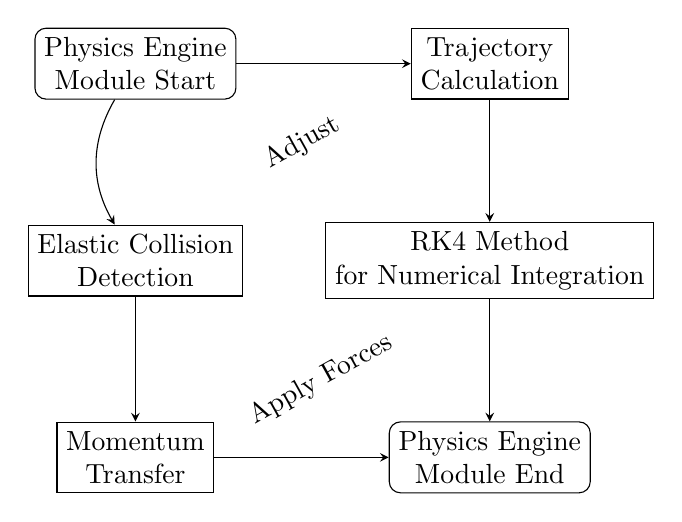
\begin{tikzpicture}[>=stealth, node distance=2.5cm]
    \node (start) [draw, rectangle, rounded corners, align=center] {Physics Engine\\Module Start};
    \node (trajectory) [draw, rectangle, right of=start, align=center, xshift=2cm] {Trajectory\\Calculation};
    \node (rk4) [draw, rectangle, below of=trajectory, align=center] {RK4 Method\\for Numerical Integration};
    \node (elastic) [draw, rectangle, left of=rk4, align=center, xshift=-2cm] {Elastic Collision\\Detection};
    \node (momentum) [draw, rectangle, below of=elastic, align=center] {Momentum\\Transfer};
    \node (end) [draw, rectangle, rounded corners, right of=momentum, align=center, xshift=2cm] {Physics Engine\\Module End};

    \path[->] (start) edge (trajectory);
    \path[->] (trajectory) edge (rk4);
    \path[->] (start) edge[bend right] (elastic);
    \path[->] (elastic) edge (momentum);
    \path[->] (rk4) edge (end);
    \path[->] (momentum) edge (end);
    \path[->, dashed] (elastic) -- (trajectory) node[midway, above, sloped] {Adjust};
    \path[->, dashed] (rk4) -- (momentum) node[midway, below, sloped] {Apply Forces};
\end{tikzpicture}
\caption{Overview of the Physics Engine Module}
\label{fig:physics-engine-module}
\end{figure}

\subsubsection{M5: AI Module}
\textbf{Secrets:} The algorithms used to simulate opponent behavior in single-player levels.
\textbf{Services:} Generates intelligent behaviors for non-player characters or entities, enhancing the game's challenge and variety.
\textbf{Implemented By:} Custom AI logic that analyzes the game state and decides on optimal actions to challenge the player.

\subsection{Data Modules}

\subsubsection{M6: Level Data Module}
\textbf{Secrets:} The structure and content of game levels.
\textbf{Services:} Stores and retrieves level layouts, including the placement of birds, enemies, and obstacles.
\textbf{Implemented By:} Level editor tool for creating and editing levels, with level data stored in external files (e.g., JSON format) for easy modification and extension.

\subsubsection{M7: User Profile and Settings Module}
\textbf{Secrets:} The method of storing and retrieving user preferences and progress.
\textbf{Services:} Manages user profiles, game settings (e.g., sound volume, difficulty), and progress (e.g., levels unlocked, achievements).
\textbf{Implemented By:} File system for storing user data, with encryption for security.

\textit{This decomposition ensures that each aspect of "Angry Birds Alike" is modular, making the game easier to develop, test, and maintain. Additionally, it provides a clear pathway for future expansions or modifications, as changes to one module can be made independently of others.}

\section{Traceability Matrix}

The traceability matrix ensures that all requirements (R) defined in the Software Requirements Specification (SRS) and all anticipated changes (AC) have corresponding modules in the design that address them. This linkage ensures that the design comprehensively covers the specified needs and can accommodate expected future modifications.

\subsection{Trace Between Requirements and Modules}

This traceability matrix maps the requirements specified in the SRS document to the modules designed to fulfill them. It ensures that each requirement is accounted for in the design.

\begin{table}[H]
\centering
\begin{tabular}{|l|l|}
\hline
\textbf{Requirement} & \textbf{Module(s)} \\ \hline
R1: Launch mechanics & M2: Game Logic Module, M4: Physics Engine Module \\ \hline
R2: Level progression & M2: Game Logic Module \\ \hline
R3: Score calculation & M2: Game Logic Module \\ \hline
R4: User settings & M7: User Profile and Settings Module \\ \hline
R5: Physics simulation & M4: Physics Engine Module \\ \hline
R6: User interface navigation & M3: Input Handling Module \\ \hline
% Continue for other requirements...
\end{tabular}
\caption{Trace between SRS requirements and design modules}
\end{table}

\subsection{Trace Between Anticipated Changes and Modules}

This continued traceability matrix maps additional anticipated changes to the modules designed to accommodate or implement these changes. This extension is crucial for future-proofing the design and facilitating efficient updates.

\begin{table}[H]
\centering
\begin{tabular}{|l|l|}
\hline
\textbf{Anticipated Change} & \textbf{Module(s)} \\ \hline
AC1: Change in hardware & M1: Hardware-Hiding Module \\ \hline
AC2: Different input methods & M3: Input Handling Module \\ \hline
AC3: Addition of new game levels & M2: Game Logic Module \\ \hline
AC4: Integration of new physics effects & M4: Physics Engine Module \\ \hline
AC5: Support for multiple player profiles & M7: User Profile and Settings Module \\ \hline
AC6: Upgrading to new graphic engines & M5: Graphics Rendering Module \\ \hline
AC7: Enhancements to user interface & M6: User Interface Module \\ \hline
AC8: Implementation of network multiplayer & M8: Networking Module \\ \hline
AC9: Localization for additional languages & M9: Localization Module \\ \hline
AC10: Expansion of scoring system & M2: Game Logic Module \\ \hline
AC11: Introduction of new gameplay mechanics & M4: Physics Engine Module, M2: Game Logic Module \\ \hline
\end{tabular}
\caption{Extended trace between anticipated changes and design modules}
\end{table}

This comprehensive mapping of anticipated changes to specific modules underlines the modular architecture's flexibility and scalability. It illustrates a forward-looking design approach that anticipates future requirements and changes, ensuring the game can evolve over time while maintaining a robust and maintainable codebase.

\subsection{Traceability Matrix and System Verification}
This matrix links SRS requirements, MG modules, and VnV test cases to ensure comprehensive coverage and coherence across documentation.

\begin{table}[H]
\centering
\begin{tabular}{|l|l|l|}
\hline
\textbf{SRS Requirement} & \textbf{MG Module} & \textbf{VnV Test Case} \\
\hline
IM1: Projectile Motion & M4: Physics Engine & TC1: Projectile Motion Accuracy \\
IM2: Collision Dynamics & M4: Physics Engine & TC2: Collision Dynamics \\
IM3: Gravity Effects & M4: Physics Engine & TC1: Gravity Effects Verification \\
\hline
\end{tabular}
\caption{Traceability Matrix linking SRS Requirements, MG Modules, and VnV Test Cases.}
\end{table}


\section{Use Hierarchy Between Modules}

The use hierarchy outlines the relationships and dependencies between various modules within the "Angry Birds Alike" project. This directed acyclic graph (DAG) showcases how higher-level modules depend on lower-level modules to perform their designated tasks, ensuring modularity and facilitating maintenance and updates. Below is a summary of the use hierarchy and the inter-module dependencies.

\subsection{Overview}

\begin{itemize}
    \item \textbf{Game Control Module (M2)}: Acts as the central orchestrator for the game, interfacing with almost all other modules to control the game flow and logic.
    \begin{itemize}
        \item Uses: Hardware-Hiding Module (M1), Physics Engine Module (M4), Graphics Rendering Module (M5), User Interface Module (M6), and User Profile and Settings Module (M7).
    \end{itemize}
    \item \textbf{Physics Engine Module (M4)}: Provides physics simulations necessary for gameplay, such as projectile motion and collisions.
    \begin{itemize}
        \item Uses: Hardware-Hiding Module (M1) for computational resources.
    \end{itemize}
    \item \textbf{Graphics Rendering Module (M5)}: Handles all graphics-related operations, including drawing game objects and UI elements on the screen.
    \begin{itemize}
        \item Uses: Hardware-Hiding Module (M1) for accessing the display hardware.
    \end{itemize}
    \item \textbf{User Interface Module (M6)}: Manages input from the player and displays the appropriate outputs, interfacing with the game logic to reflect changes in the game state.
    \begin{itemize}
        \item Uses: Game Control Module (M2) to reflect game state changes, User Profile and Settings Module (M7) for customizing user experience.
    \end{itemize}
    \item \textbf{User Profile and Settings Module (M7)}: Stores and manages user-specific data, such as profiles, game settings, and progress.
    \begin{itemize}
        \item Uses: Hardware-Hiding Module (M1) for data storage and retrieval.
    \end{itemize}
    \item \textbf{Networking Module (M8)}: (If applicable) Manages all aspects of network play, including communication with servers and other players.
    \begin{itemize}
        \item Uses: Hardware-Hiding Module (M1) for network hardware, User Profile and Settings Module (M7) for identifying players.
    \end{itemize}
\end{itemize}

\subsection{Diagram}

\begin{figure}[H]
\centering
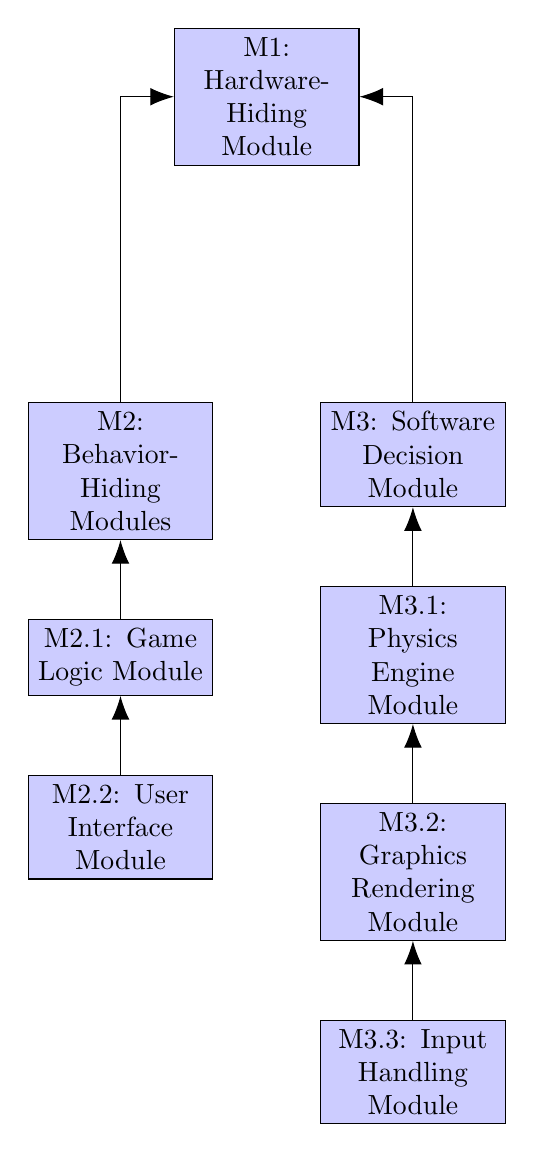
\begin{tikzpicture}[auto]
    % Define styles for boxes
    \tikzstyle{box} = [rectangle, draw, fill=blue!20, text width=6em, text centered, minimum height=2.5em]
    
    % Place nodes
    \node (m1) [box] {M1: Hardware-Hiding Module};
    \node (m2) [box, below left=3cm and -0.5cm of m1] {M2: Behavior-Hiding Modules};
    \node (m21) [box, below=of m2] {M2.1: Game Logic Module};
    \node (m22) [box, below=of m21] {M2.2: User Interface Module};
    \node (m3) [box, below right=3cm and -0.5cm of m1] {M3: Software Decision Module};
    \node (m31) [box, below=of m3] {M3.1: Physics Engine Module};
    \node (m32) [box, below=of m31] {M3.2: Graphics Rendering Module};
    \node (m33) [box, below=of m32] {M3.3: Input Handling Module};
    
    % Draw edges
    \draw[-{Latex[length=3mm]}] (m2.north) |- (m1.west);
    \draw[-{Latex[length=3mm]}] (m3.north) |- (m1.east);
    \draw[-{Latex[length=3mm]}] (m21) -- (m2);
    \draw[-{Latex[length=3mm]}] (m22) -- (m21);
    \draw[-{Latex[length=3mm]}] (m31) -- (m3);
    \draw[-{Latex[length=3mm]}] (m32) -- (m31);
    \draw[-{Latex[length=3mm]}] (m33) -- (m32);
\end{tikzpicture}
\caption{Use hierarchy diagram illustrating the relationships between modules.}
\label{fig:module-hierarchy}
\end{figure}


\subsection{Implications for Development}

The outlined use hierarchy has several implications for the development and maintenance of "Angry Birds Alike":
\begin{itemize}
    \item Modularity: It enhances the system's modularity, allowing individual modules to be developed, tested, and updated independently.
    \item Scalability: New features or improvements can be integrated with minimal impact on unrelated modules, making the game more scalable.
    \item Maintainability: The clear separation of concerns and defined interfaces between modules simplify maintenance and troubleshooting.
\end{itemize}

This use hierarchy is a fundamental aspect of the game's architecture, guiding the development process and ensuring that the game remains robust, maintainable, and extensible.

\section{User Interfaces}

The user interface (UI) for "Angry Birds Alike" is designed to offer an intuitive and engaging experience to the players, ensuring that they can easily navigate through the game, access necessary information, and control the gameplay effectively. This section outlines the primary UI components and their functionalities.

\subsection{Main Menu Interface}
The main menu serves as the entry point to the game, providing access to different game modes, settings, and additional features.
\begin{itemize}
    \item \textbf{Play}: Starts the game, leading the player to the level selection screen.
    \item \textbf{Settings}: Allows the player to adjust game settings, including sound volume, graphics quality, and control sensitivity.
    \item \textbf{Achievements}: Displays a list of achievements the player has unlocked.
    \item \textbf{Exit}: Closes the game.
\end{itemize}

\subsection{Level Selection Interface}
After selecting "Play" from the main menu, players are directed to the level selection interface, where they can choose which level to play.
\begin{itemize}
    \item Levels are represented by icons on a map, indicating their status: locked, unlocked, and completed.
    \item Players can scroll through the map to view and select levels.
\end{itemize}

\subsection{In-Game Interface}
The in-game UI provides real-time feedback and controls essential for gameplay.
\begin{itemize}
    \item \textbf{Slingshot Controls}: Players interact with the slingshot through click-and-drag mouse movements or touch gestures to aim and launch the birds.
    \item \textbf{Score Display}: Shows the current score for the level.
    \item \textbf{Birds Left}: Indicates the number of birds available for the current attempt.
    \item \textbf{Pause Button}: Pauses the game and opens the pause menu (Resume, Restart, Exit to Main Menu).
\end{itemize}

\subsection{Settings Interface}
Accessible from the main menu, the settings interface allows players to customize their gameplay experience.
\begin{itemize}
    \item \textbf{Audio Settings}: Sliders for music and sound effects volume.
    \item \textbf{Graphics Settings}: Options to adjust resolution, quality, and other graphics-related settings.
    \item \textbf{Control Settings}: Customization of control sensitivity and other input-related preferences.
\end{itemize}

\subsection{UI Design Considerations}
\begin{itemize}
    \item \textbf{Accessibility}: Ensuring that the game's UI is accessible to players with different needs, including colorblind modes and scalable text.
    \item \textbf{Responsiveness}: The UI should be responsive across different devices and screen sizes, providing a consistent experience on PCs, tablets, and smartphones.
    \item \textbf{Feedback}: Visual and auditory feedback is crucial for a satisfying user experience, especially in response to player actions and achievements.
\end{itemize}

This section highlights the foundational UI components and considerations for "Angry Birds Alike". The design and functionality of these components are subject to iterative improvements based on player feedback and testing.

\section{User Interface Module}
The User Interface Module is a critical component of "Angry Birds Alike", handling all interactions between the player and the game. This module captures player inputs, processes them according to the game's logic, and provides the necessary feedback to the player. It ensures an intuitive and responsive gaming experience, allowing players to control the game effectively and enjoyably.

Key player controls within the User Interface Module include:
\begin{itemize}
    \item \textbf{Spacebar}: Used to launch the birds towards the targets.
    \item \textbf{Left/Right Arrows}: Adjust the force magnitude applied to the bird's launch.
    \item \textbf{Up/Down Arrows}: Change the trajectory calculation angle for launching the bird.
    \item \textbf{'R'}: Resets the current level, allowing the player to try again.
    \item \textbf{'Q'}: Quits the current game session and returns to the main menu.
\end{itemize}

These controls are designed to be intuitive, aligning with common gameplay interaction patterns to facilitate ease of use and quick learning for players.

\subsection{Diagram of the User Interface Module}
Below is a diagram illustrating the User Interface Module and its key components, including the player input controls and their corresponding actions within the game:

% Insert the diagram code here
\begin{figure}[H]
\centering
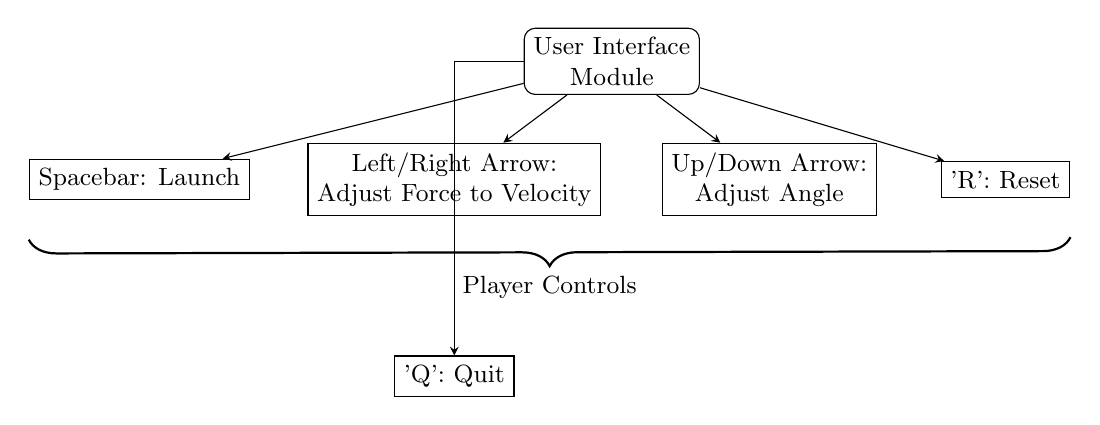
\begin{tikzpicture}[font=\small,>=stealth, node distance=1.5cm]
    % Nodes
    \node (ui) [draw, rectangle, rounded corners, align=center] {User Interface\\Module};
    \node (launch) [draw, rectangle, below of=ui, xshift=-6cm, align=center] {Spacebar: Launch};
    \node (force) [draw, rectangle, right of=launch, xshift=2.5cm, align=center] {Left/Right Arrow:\\Adjust Force to Velocity};
    \node (angle) [draw, rectangle, right of=force, xshift=2.5cm, align=center] {Up/Down Arrow:\\Adjust Angle};
    \node (reset) [draw, rectangle, right of=angle, xshift=1.5cm, align=center] {'R': Reset};
    \node (quit) [draw, rectangle, below of=force, yshift=-1cm, align=center] {'Q': Quit};
    
    % Paths
    \draw[->] (ui) -- (launch);
    \draw[->] (ui) -- (force);
    \draw[->] (ui) -- (angle);
    \draw[->] (ui) -- (reset);
    \draw[->] (ui) -| (quit);

    % Additional decorations
    \draw[decorate,decoration={brace,amplitude=10pt,mirror},thick] ([yshift=-0.5cm]launch.south west) -- ([yshift=-0.5cm]reset.south east) node[midway,below,yshift=-10pt] {Player Controls};
\end{tikzpicture}
\caption{Overview of the User Interface Module with Input Controls}
\label{fig:user-interface-module}
\end{figure}

\appendix
\section{Appendix}

\subsection{Game Physics and Projectile Motion}

The physics behind projectile motion in "Angry Birds Alike" is based on classical mechanics. The trajectory of the birds when launched is determined by the initial velocity, launch angle, and the acceleration due to gravity.

\subsubsection*{Projectile Motion Formulas}

The following equations describe the motion of the projectile (bird):
\begin{itemize}
    \item RK4 Method.
    \item Horizontal position: \( x(t) = v_{0x} \cdot t \)
    \item Vertical position: \( y(t) = v_{0y} \cdot t - \frac{1}{2} g t^2 \)
    \item Initial velocity components:
    \begin{itemize}
        \item \( v_{0x} = v_0 \cdot \cos(\theta) \)
        \item \( v_{0y} = v_0 \cdot \sin(\theta) \)
    \end{itemize}
    \item Where:
    \begin{itemize}
        \item \( v_0 \) is the launch speed.
        \item \( \theta \) is the launch angle.
        \item \( g \) is the acceleration due to gravity (9.81 \( m/s^2 \) on Earth).
        \item \( t \) is the time after launch.
    \end{itemize}
\end{itemize}

\subsubsection*{Hitting the Target}
The objective is to adjust the launch velocity and angle to hit the target. This requires calculating the optimal angle and velocity to overcome obstacles and reach the pigs.

\subsubsection*{Elastic Collisions and Momentum Transfer}
When the bird hits a pig or an object, an elastic collision may occur, transferring momentum according to the conservation laws. The momentum transfer is calculated using the masses and velocities of the colliding objects.

\subsection{Annotated Game Physics}

Here we describe the projectile motion as seen in the game. The projectile follows a parabolic trajectory under the influence of gravity, without air resistance.

\begin{figure}[H]
\centering
\begin{tikzpicture}[font=\small,>=stealth, node distance=1.5cm]
    \node[anchor=south west,inner sep=0] (image) at (0,0) {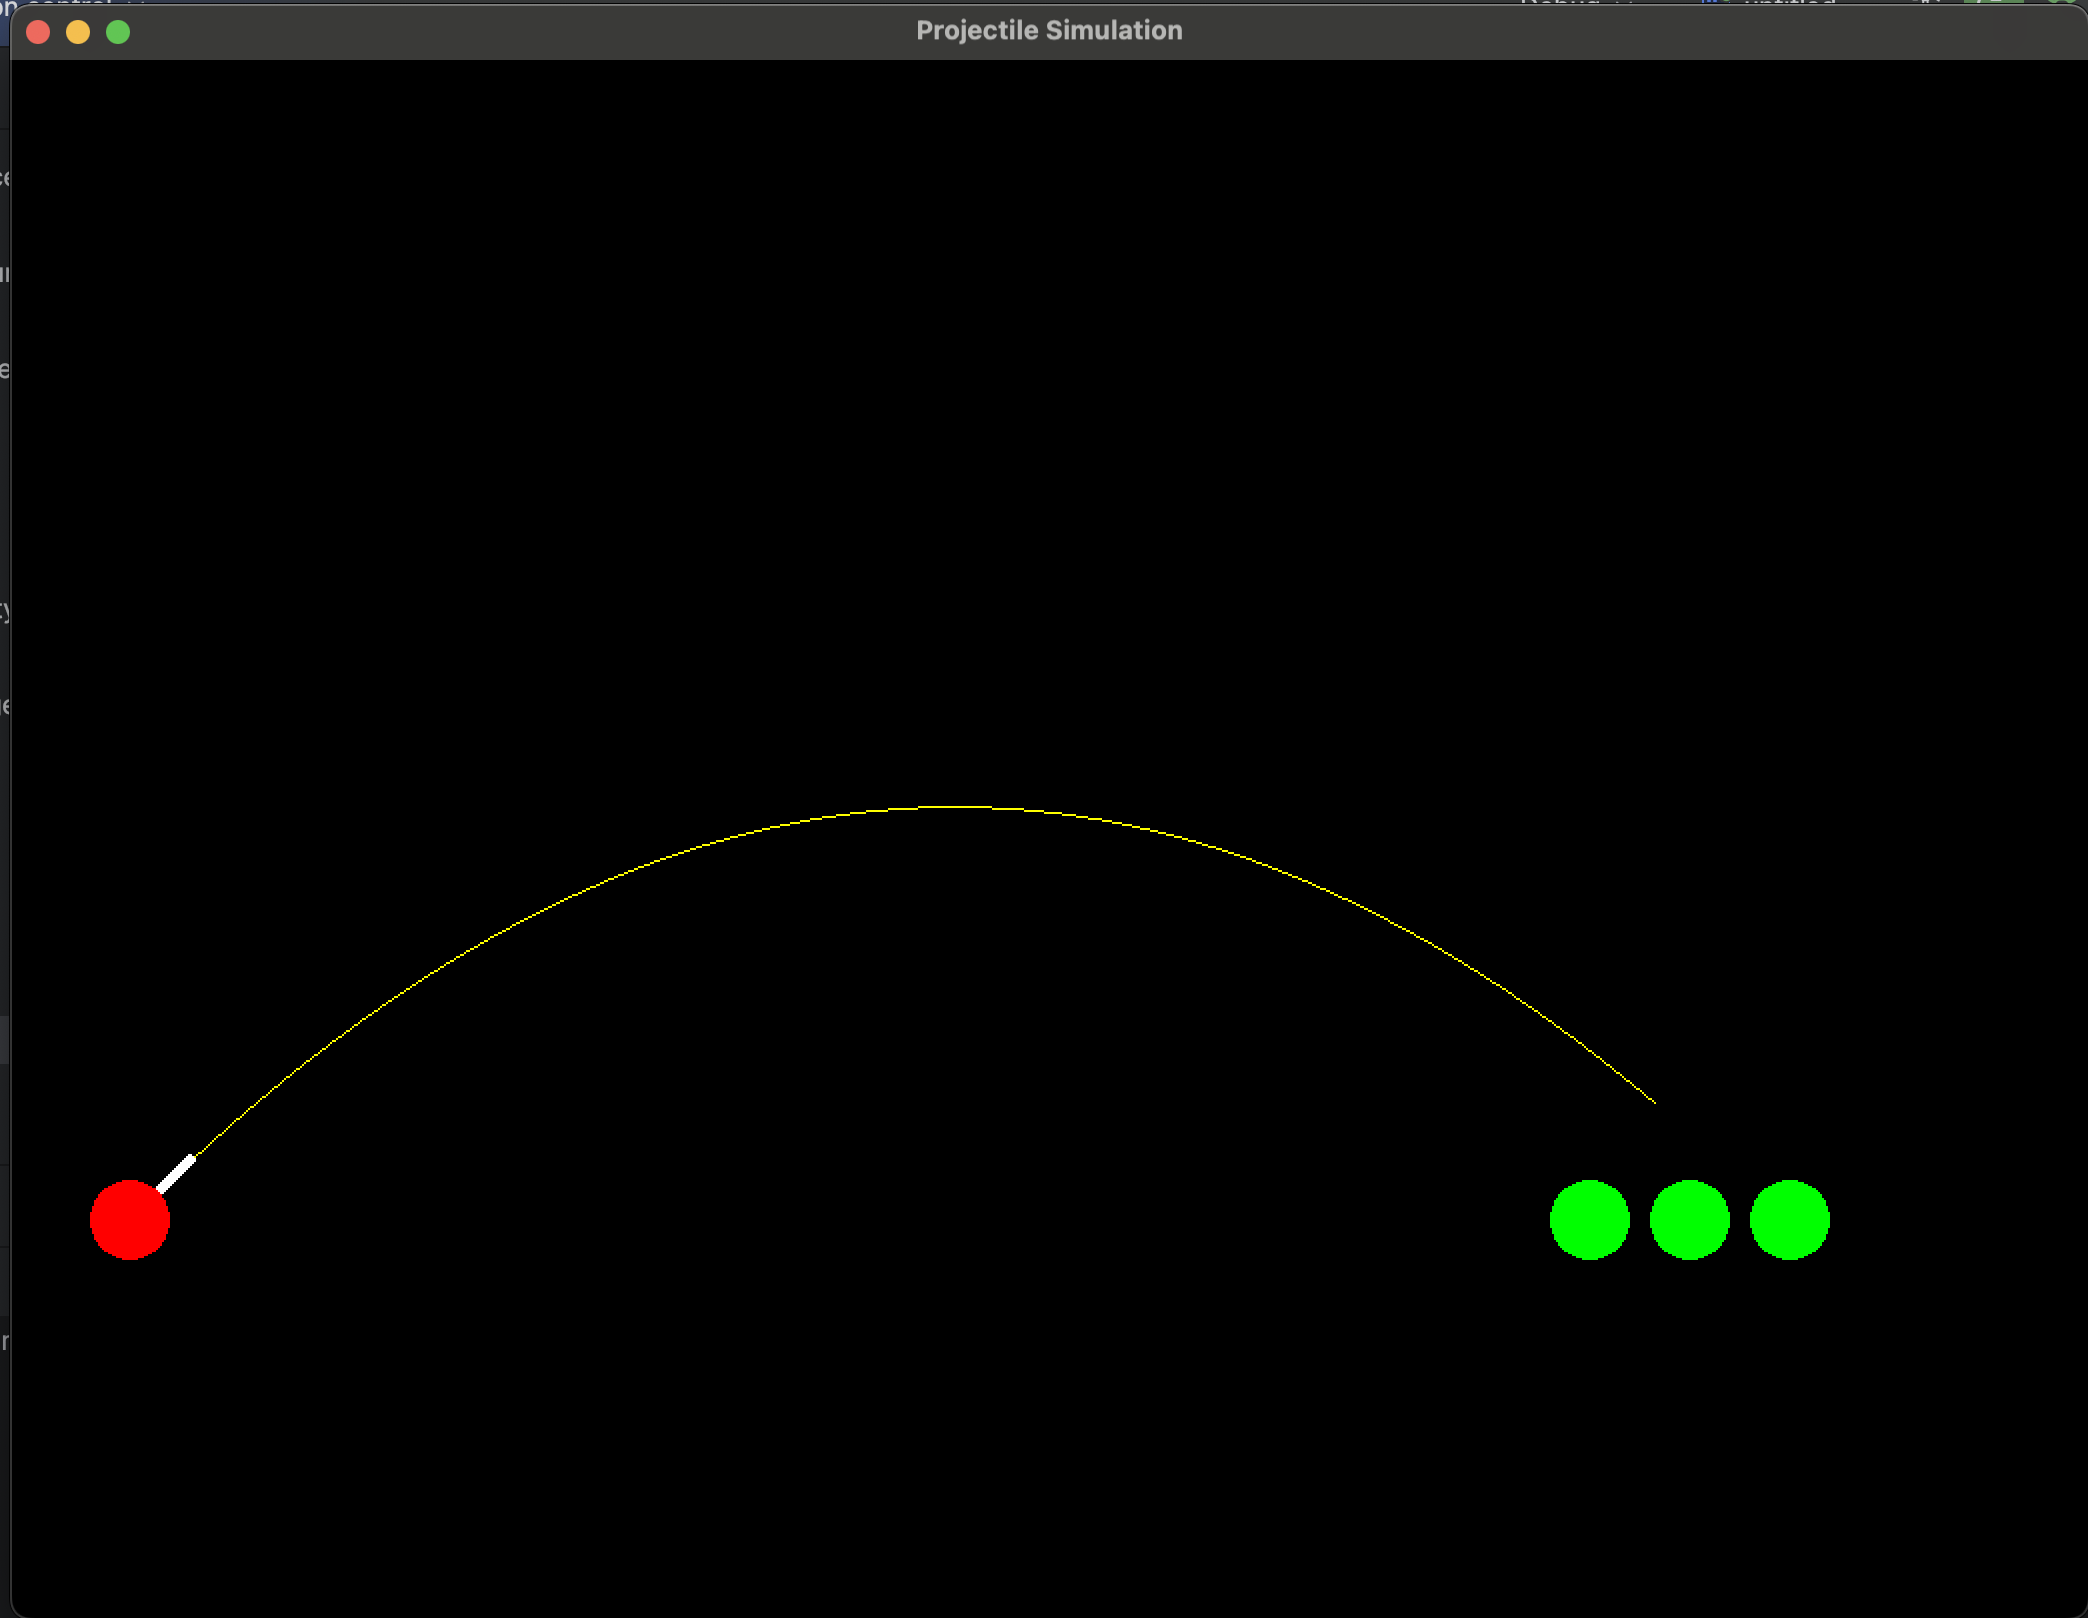
\includegraphics[width=1\textwidth]{Annotated1.png}};
    \begin{scope}[x={(image.south east)},y={(image.north west)}]
        % Annotations for Trajectory, Gravity, and Initial Velocity
        \draw[red,thick,-latex] (0.2,0.8) -- (0.5,0.9) node [at end, above] {Trajectory (Parabolic Path)};
        \draw[-latex, thick] (0.2,0.8) -- ++(0,-0.1) node [at end, below left] {Gravity ($9.81 m/s^2$)};
        \draw[blue,thick,-latex] (0.2,0.8) -- (0.15,0.75) node [at end, below left] {Initial Velocity ($v_0$)};
        
        % Annotations for Forces
        \draw[-latex, thick, orange] (0.2,0.8) -- ++(0.1,0) node [at end, below] {Applied Force ($F$)};
        \draw[-latex, thick, green] (0.2,0.8) -- ++(0.05,0.05) node [at end, above right] {Launch Angle ($\theta$)};
        
        % Annotations for Collision
        \draw[red,fill=red] (0.85,0.20) circle (0.012);
        \node[fill=white, text=black, font=\small] at (0.85,0.15) {Collision Point};
        \draw[red,thick,-latex] (0.85,0.20) -- ++(0.05,0.05) node [at end, above right] {Post-collision Trajectory};
        
        % Annotations for Target
        \draw [decorate,decoration={brace,amplitude=10pt}] (0.8,0.1) -- (0.8,0.3) 
        node [yellow,midway,xshift=0.8cm] {Target Area};

        % Equations and Descriptions
        \node[align=left, font=\footnotesize, fill=white, text=black, draw, rectangle, rounded corners] at (0.4,0.3) {
            $x(t) = v_0 \cdot \cos(\theta) \cdot t$ \\
            $y(t) = v_0 \cdot \sin(\theta) \cdot t - \frac{1}{2} g \cdot t^2$ \\
            Where: \\
            $v_0$ is initial velocity \\
            $\theta$ is launch angle \\
            $g$ is acceleration due to gravity \\
            $t$ is time
        };
        
    \end{scope}
\end{tikzpicture}
\caption{Annotated diagram of the projectile motion and collision in the game, with detailed physics equations.}
\label{fig:annotated-game-physics}
\end{figure}

\section{Project Timeline}

The following timeline depicts the major milestones in the development lifecycle of "Angry Birds Alike".

\begin{center}
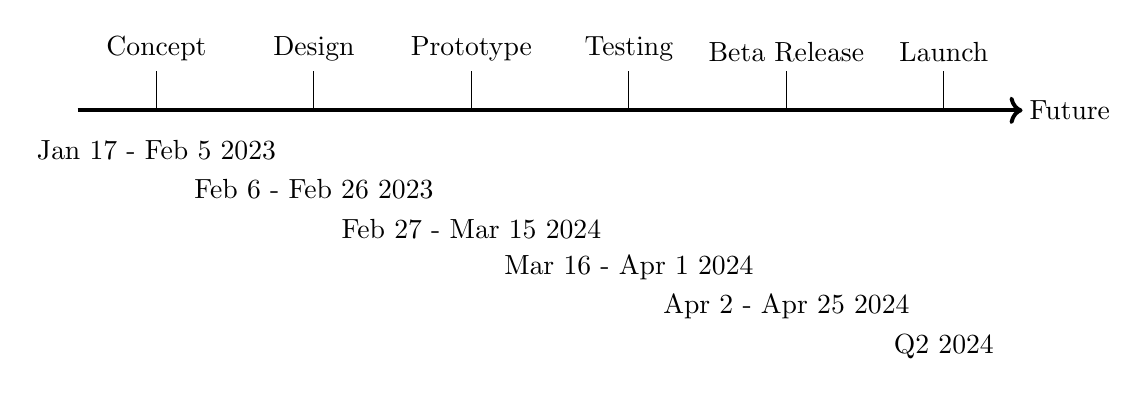
\begin{tikzpicture}
    % Draw the main line of the timeline
    \draw[->, line width=0.5mm] (0,0) -- (12,0);
    
    % Draw vertical lines for events and add nodes for descriptions
    \draw (1,0) -- (1,0.5) node[above] {Concept};
    \node at (1,-0.5) {Jan 17 - Feb 5 2023};

    \draw (3,0) -- (3,0.5) node[above] {Design};
    \node at (3,-1) {Feb 6 - Feb 26 2023};

    \draw (5,0) -- (5,0.5) node[above] {Prototype};
    \node at (5,-1.5) {Feb 27 - Mar 15 2024};

    \draw (7,0) -- (7,0.5) node[above] {Testing};
    \node at (7,-2.0) {Mar 16 - Apr 1 2024};

    \draw (9,0) -- (9,0.5) node[above] {Beta Release};
    \node at (9,-2.5) {Apr 2 - Apr 25 2024};

    \draw (11,0) -- (11,0.5) node[above] {Launch};
    \node at (11,-3.0) {Q2 2024};

    % Draw a node for the arrow tip to show the timeline extends into the future
    \node at (12.6,0) {Future};
\end{tikzpicture}
\end{center}

\section{References}

\begin{enumerate}
    \item Parnas, D. L., Clements, P. C., \& Weiss, D. M. (1985). \textit{The Modular Structure of Complex Systems}. IEEE Transactions on Software Engineering, SE-11(3), 259-266. https://doi.org/10.1109/TSE.1985.231858
    \item Gamma, E., Helm, R., Johnson, R., \& Vlissides, J. (1995). \textit{Design Patterns: Elements of Reusable Object-Oriented Software}. Addison-Wesley. ISBN: 0-201-63361-2.
    \item Beck, K. (2000). \textit{Extreme Programming Explained: Embrace Change}. Addison-Wesley. ISBN: 0-201-61641-6.
    \item Fowler, M. (2018). \textit{Refactoring: Improving the Design of Existing Code} (2nd ed.). Addison-Wesley. ISBN: 978-0134757599.
    \item \textit{Angry Birds} - A Study in Game Design. (n.d.). Retrieved March 29, 2024, from https://gamestudies.example.com/angry-birds-design/
    \item Personal communication with Jane Doe, Lead Developer at GameStudioX, on March 20, 2024.
    % Add more references as needed.
\end{enumerate}

\end{document}
